% (c) 2020 Stefan Antonowicz
% Based off of tex found at https://github.com/ludus-leonis/nipajin
% This file is released under Creative Commons Attribution-NonCommercial-ShareAlike 4.0 International License.
% Please do not apply other licenses one-way.

\renewcommand{\yggMechanics}{%
  \mychapter{Core Mechanics}{core-mechanics}
}

\renewcommand{\yggMechanicsText}{%

  \end{multicols}

  \mybold{Important: this book is supplemental to the Core Rules - read that book first!}

  \mysection{Abbreviations}{abbreviations}

  \example{
    \mylist {
      \item \hrulefill
      \item \DICE\bgspace The number of dice used to cast the spell 
      \item \hrulefill
      \item \SUMDICE\bgspace The sum of the dice used in casting the spell
      \item \hrulefill
      \item \MOD\bgspace A modifier to the roll you make. Can be positive or negative.
      \item \hrulefill
      \item \DURATION\bgspace The Duration of the spell - a length of time (Combat, \SUM Minutes, Session, etc); Concentration; or Markovian)
      \item \hrulefill
      \item \LENGTH\bgspace The length of time it takes you to perform a spell or ability.  Default is 1 Maneuver
      \item \hrulefill
      \item \COST\bgspace The number and type of coins worth of materials required for the spell, ritual, etc. If the type of coin isn't specified (iron, silver, or gold) it will be the coin appropriate for the Civilization (small, medium, or large)
      \item \hrulefill
      \item \TARGET\bgspace Who or what you can target, and how far away
      \item \hrulefill
      \item \COUNTER\bgspace If the spell can be countered by another spell (and if so, what spell counters it).
      \item \hrulefill
      \item \PARADIGM\bgspace  The Paradigm of the spell - what kinds of spell it is
      \item \hrulefill
      \item \REVERSE\bgspace If the spell or effect is reversible (that is, if an opposite version of the spell might be cast i.e.  Heal vs. Harm, etc)
      \item \hrulefill
      \item \KEYWORD\bgspace Any Keyword(s) associated with the spell
      \item \hrulefill
      \item \SAVE\bgspace Whether or not a victim gets a Save vs. Hexes (Yes or No).  The result of a successful Save will be in the spell's description

    }
  }

  \newpage 

  \begin{multicols}{2}\raggedcolumns

  \mysection{Duration}{duration}

  \mysubsection{Markovian}{duration-markovian}
  
  Markovian spells take effect immediately, but have a random duration depending on the number of dice \DICE invested in the casting:

  \mytable{>{\centering\arraybackslash}X  X} {
    \thead{\DICE} & {Duration} \\
  } {
    1 & d4 \\
    2 & d6 \\
    3 & d8 \\
    4 & d10 \\
    5 & d12 \\
    6+ & d16 \\
  }

  At the top of the Moment, roll an \RS with the appropriate die.  If you fail (a 1 or a 2), the Markovian effect ends.  If you succeed, the die moves \DCDOWN


  \mysubsection{Concentration}{duration-concentration}
  
  Some Arcana require \mybold{Concentration} to maintain.  Concentration is broken if: (a) the target moves out of range or line of sight, or (b) the adventurer maintaining the Concentration is distracted. Distraction is at the Arbiter's discretion - taking damage, being affected by the environment or by a spell, getting knocked over, etc.  The adventurer maintaining the Concentration can walk slowly and still Concentrate, but cannot run.  They can whisper but not speak or yell.  The adventurer can voluntarily end a Concentration arcana at any time.

  \mysubsection{Other}{duration-other}

  \mylist {
    \item A duration of \mybold{Combat} indicates a spell or effect that will end at the end of Combat, before you take a Breather. \\~ \\~

    \item A duration of \mybold{\SUM Minutes} indicates a spell or effect that will last a number of real world minutes as shown on the di(c)e.  The Arbiter should use a stopwatch or clock to measure the passage of time.  The adventurer can ask how many minutes are left at any time and get an answer, but the Arbiter is under no obligation to volunteer how much time remains if she doesn't want to. \\~ \\~

    \item A duration of \mybold{Session} means the spell lasts for the entire Session.  It will need to be recast at the start of the next Session if you want the effect to continue.
  }

  \mysection{Keywords}{keywords}

  \mysubsection{Contested}{keyword-contested}

  Contested spells are a \RB between the spell caster and a Monster.  The caster's \RB is their Primary Stat ( \INT for Philosophers, \FOC for Mystics, and Awareness for Spriggan).  The target's \RB will be defined in the spell.  
  \example{
    The Wizardry arcanum \mylink{Battering Beam}{wizardry-battering-beam} is a \RB between the Philospher's \INT and the target's \VIG with a -\DICE penalty.  The Philosopher will \RB : \INT + \LVL (since Philosophers add their level to any \INT rolls), and the victim will need to \RB : \VIG - \DICE, plus any other modifiers. 
  }

  \mysubsection{Splittable}{keyword-splittable}

  Spells that can be split can have their dice split up among up to \DICE targets.  Each target resolves the effect of the dice on them separately, but the \DICE are pooled when considering Mishaps, Calamities, and Ruin.

  \example {
    The Wizardry arcanum \mylink{Charm}{wizardry-charm} is Splittable and allows you to "...[e]nsorcel one or more Monsters whose \HD are less than or equal to \DICE". If you had a pool of 4 Blood Dice, you could use 3 [dice] on 1 Monster and 2 on another, 1 [die] on 4 Monsters, etc. with the additional requirement that the \DICE used on the Monster is equal to or greater than their \HD
  }

 \newpage

  \mysubsection{Hammerspace}{keyword-hammerspace}
  \flavor {
    "... a fan-envisioned extradimensional, instantly accessible storage area in fiction, which is used to explain how animated, comic, and game characters can produce objects out of thin air." 
  }

  Arcana that make use of Hammerspace allow you to place objects in an "out of game" area until they can be retrieved.  Hammerspace objects can't be stolen, used, or obtained by others - but certain other arcana can tell unsavories whether or not you have things stored in Hammerspace.  You can't put one Hammerspace object in another (they repel like magnets). Objects in Hammerspace immediately return to reality when you die.  No one is really 100\% on how long a living thing can survive in Hammerspace.  

\cbreak

  \mysubsection{Purge}{keyword-purge}
  
  When something is "purged", it removes permanent effects in addition to temporary effects.  For example, the Leechcraft of \mylink{Bonesetting}{leechcraft-bonesetting} purges a non-serious Physical wound.  

  \begin{center}
  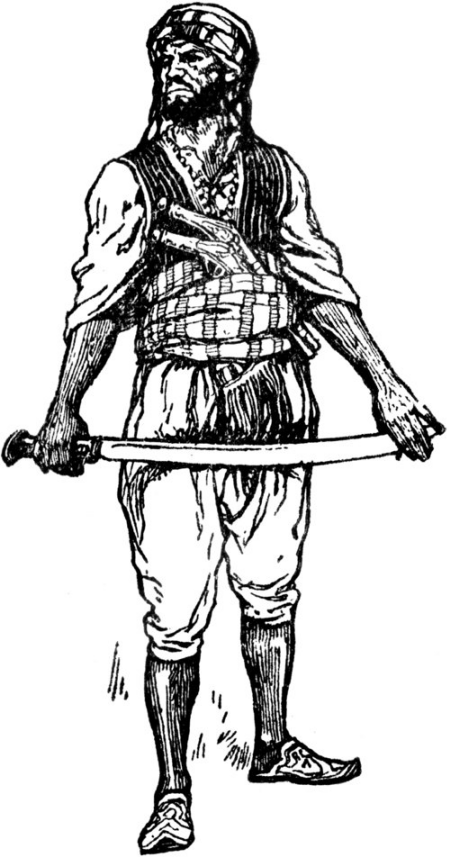
\includegraphics[scale=.5]{Warrior}
  \end{center}


  \newpage

  \mysection{Mortals}{mortals}

  Mortals are marked by the sign of Kib, and blessed with a soul (the \myital{noumenon}, the "thing in itself").  The existence of this soul means you are Hallowed, one of the chosen members of the sacred Tribes of \TheAuthority.  All Hallowed things stand in opposition to Magic, a phenomenon whose rules are bound in Chaos rather than Order. Only through the manipulation of the \mybold{Four Cruces} are the Hallowed able to understand the \mylink{Arcana}{arcana} denied to them by the Sign of Kib.

  \mysubsection{The Four Cruces}{mortals-four-cruces}

  \myhighlight{Blood}{mortal-crux-blood}

  The \mylink{Crux of Blood}{philosopher-crux-blood} allows Mortals to shape Magic in its raw form, the hand shaping the clay into a vessel. Blood allows Mortals to practice \mylink{Wizardry}{philosopher-wizardry}.

  \myhighlight{Faith}{mortal-crux-faith}

  The \mylink{Crux of Faith}{mystic-crux-faith} is the conduit to the Small Gods, the kitestring of the kite that rides the winds of heaven.  Faith allows Mortals to perform \mylink{Liturgies}{mystics-liturgies}.


  \myhighlight{Knowledge}{mortal-crux-knowledge}

  The \mylink{Crux of Knowledge}{philosopher-crux-knowledge} are the nourishing fruits of the Tree of Ygg, the fuel of the fire of Mortality.  Knowledge opens the door to \mylink{Leechcraft}{philosopher-leechcraft}.

  \myhighlight{Mojo}{mortal-crux-mojo}

  The \mylink{Crux of Mojo}{mystic-crux-mojo}  is the yielding to Magic to both wield and be wielded by its Arcana, like yielding to a lover's embrace. Mojo allows Mortals to affect reality directly, including cheating death through \mylink{Necromancy}{arcana-necromancy}

    \cbreak
  \mysection{Unseelie}{unseelie}

  The Unseelie races are \myital{phenomenal} - they lack a definable essence, since they are born of Magic and Chaos (though they stand outside of it in the same way a fish swimming in a stream is both a part of and separate from the water). The Unseelie exist so long as Magic exists. They are unmarked by \TheAuthority (like familiars, constructs, and the undead), and thus stand in opposition to Mortals. For this reason they are considered Unhallowed.  Through the \mylink{Gift of Grace}{mystic-grace}, Mortals can banish the Unhallowed from their midst.


} %end
